%\documentclass{sig-alternate}
\documentclass[12pt]{article}
\usepackage{graphicx}
\usepackage{pifont}
\usepackage{url}
\usepackage{code}
\usepackage{amsmath}
\usepackage{algpseudocode} 
\usepackage{algorithmicx}
\usepackage{algorithm}
\usepackage{xcolor}
\usepackage{setspace}
\usepackage[margin=1in]{geometry}
%\usepackage{flushend}

\newcommand{\mycomment}[1]{}

%\setcopyright{usgov}
%\setcopyright{usgovmixed}
%\setcopyright{cagov}
%\setcopyright{cagovmixed}

\doublespacing

% DOI
%\acmDOI{10.475/123_4}

% ISBN
%\acmISBN{123-4567-24-567/08/06}

%%% The following is specific to TECPS'17 and the paper
%%% 'Towards Automated Composition of Heterogeneous Tests for Cyber-Physical Systems'
%%% by Alex Groce, Paul Flikkema, and Josie Holmes.
%%%


\begin{document}

\pagenumbering{roman}

\title{Section A\\Title: Automated Composition of Tests for
  Cyber-Physical Systems\\
\small{BAA FA8750-17-S-7007 Topic 5(c)}}
%\title{Normalizing and Generalizing Test Cases}

\author{Alex Groce and Paul Flikkema\\
School of Informatics, Computing, and Cyber Systems \\
  Northern Arizona University, USA}

%\numberofauthors{3}

%\alignauthor
%Alex Groce\\
%       \affaddr{School of Electrical Engineering and Computer Science}\\
%       \affaddr{Oregon State University}\\
%       \email{agroce@gmail.com}
% 2nd. author
%\alignauthor
%Josie Holmes\\
%       \affaddr{Department of Geography}\\
%       \affaddr{Pennsylvania State University}\\
%       \email{webmaster@marysville-ohio.com}
% 3rd. author
%\alignauthor Kevin Kellar\\
%       \affaddr{Crescent Valley High School}\\
%       \affaddr{1 Th{\o}rv{\"a}ld Circle}\\
%      \affaddr{Hekla, Iceland}\\
%      \email{larst@affiliation.org}
%}


%\begin{abstract}
%A key trait of modern cyber-physical systems (CPS) is complexity due to the number of components and layers in these systems.  Unlike in traditional software development, where the device layer is essentially completely abstracted away by an operating system, CPS components include low-power edge nodes, gateways, and servers that together provide sensing, actuation, communication, model and state inference, and autonomous or user-driven control.  Moreover, the CPS design process involves implementation of these functions at different levels of abstraction, from high-level computational models to bare-mental implementations. Unfortunately, even when advanced testing or verification methods are applied only to low level system aspects, those efforts are separated from high-level tests of a CPS, which are often produced by a different team, and do not stress the low-level system.  Effective automated test composition would make it possible to automatically produce integration/system tests for CPS, even with extremely heterogeneous aspects, where individual elements have effective tests but the interactions between the sub-systems are untested.  Because of the size of the search space involved and the complexity of modeling and designing CPS, we also propose in the long term a move towards system architectures to support testing across both system layers and levels of abstraction.

%\end{abstract}

\mycomment{

\author{\IEEEauthorblockN{%
Alex Groce,\IEEEauthorrefmark{1}
Josie Holmes\IEEEauthorrefmark{2}
Kevin Kellar\IEEEauthorrefmark{3}
}

\IEEEauthorblockA{\IEEEauthorrefmark{1}%
School of Electrical Engineering and Computer Science\\
Oregon State University\\
\IEEEauthorrefmark{2}
Department of Geography\\
Pennsylvania State University
\IEEEauthorrefmark{3}
Crescent Valley High School
}


}
%\author{\IEEEauthorblockN{Alex Groce, Amin Alipour, Chaoqiang Zhang, Yang Chen, John Regehr}
%\IEEEauthorblockA{School of Electrical Engineering and Computer Science\\
%Oregon State University, Corvallis, OR\\
%Email: agroce@gmail.com, alipourm,zhangch@onid.oregonstate.edu}}
}

\mycomment{
\numberofauthors{1}
\author{
\alignauthor
Arpit Christi, Matthew Lyle Olson, Mohammad Amin Alipour, Alex Groce\\
\affaddr{School of Electrical Engineering and Computer Science}\\
\affaddr{Oregon State University}
\affaddr{Corvallis, OR USA}\\
%\affaddr{Corvallis, OR}\\
%\affaddr{USA}
}
}

\maketitle

\noindent{\bf Period of Performance:} September 15, 2018 - September
14, 2021\\
\vspace{0.1in}\\
{\bf Estimated Cost:} \$336,634\\
\vspace{0.1in}\\
{\bf Name/Address of Company:}\\
Northern Arizona University\\
School of Informatics, Computing, and Cyber Systems (Bldg \#90, floors 1 and 2)\\
1295 S. Knoles Drive \\
PO Box 5693 \\
Flagstaff, AZ 86011\\
\newpage
\noindent{\bf Technical Points of Contact:}\\
Alex Groce\\
phone: 1 928 523-8263\\
fax: 1 928 523-1902\\
email: {\tt alex.groce@nau.edu}\\
Paul Flikkema\\
phone: 1 928 523-6114\\
fax: 1 928 523-1902\\
email: {\tt paul.flikkema@nau.edu}\\
\vspace{0.05in}\\
{\bf Contracting Point of Contact:}\\
Kay McConagha\\
phone: 1 928 523-8752\\
fax: 1 928 523-1902\\
email: {\tt kay.mcconagha@nau.edu}
\vspace{1in}\\
CAGE Code: UNKNOWN\\
Unique Entity Identifier:  UNKNOWN\\


\newpage
\pagenumbering{arabic}
\section{B:  Task Objective}

The objective of this task is to develop methods and tools for composing tests for
(potentially heterogenous) components of a cyber-physical system
(CPS). \mycomment{
Composition of existing tests enhances the utility of formal
verification, automated testing, and manual testing driven by systems
engineers, human interface experts, or quality-assurance experts.
Composition of tests also provides a novel test generation method that
can detect previously un-detected faults arising from interactions of
system components tested using disparate methods.}

\section{C: Technical Summary and Proposed Deliverables}

Modern cyber-physical systems (CPS) design employs layering in multiple domains, e.g., computation, networking, and the modeling of the embedding physical system and the system's sensors and actuators. However, current layering approaches do not capture non-functional system properties essential to CPS, e.g., timing and energy use, that emerge via testing.  To manage design process complexity, iterative development is commonplace: while the long-term trend is refinement of abstract models, engineers often need to shift back and forth between implementation-level models and more abstract models to gather new data, gain knowledge and insight, and optimize system performance.

The same multiplicity of heterogeneous layers also often applies to existing tests for complex systems: often components of a system, such as a file system or actuators, are tested by one set of engineers, and using completely different methods than are used to produce tests at the high level of either control software with humans-in-the-loop or autonomous control systems.  The core functionality of a system is usually written in low-level, embedded systems languages, such as C.  In the ideal case, such systems are developed using both formal specification and verification and sophisticated automated testing.  In some cases the formal specification is used to generate executable tests to ensure the real system matches the formal models; in other cases there is at least a very determined test generation effort, including efforts to produce very high-coverage tests.  In contrast, user-centric or high-level autonomy layers are often developed in higher-level languages, such as Java, and with a much more informal approach to testing and verification.  Increasingly, mission- and safety-critical low-level elements interact with users or high-level autonomy.  Even when the behavior of each system, in isolation, is valid, the composition may compromise performance, user experience, security and privacy, or (in the worst case) safety.

Existing tests for different layers are highly valuable; however, they typically fail to cover the interaction of components effectively.  This problem is made worse by a fundamental limitation: tests do not compose.  Even within a single system, executing test {\tt A} followed by test {\tt B} seldom produces the desired union of behaviors (e.g., even covering all code covered by {\tt A} or {\tt B}).  The actions of {\tt A} often interfere with those of {\tt B} (or vice versa): that is, some action in {\tt A} is either illegal in a composed context, causing {\tt B} (and thus the entire test) to become invalid, or disables some behavior of {\tt B}, lowering test effectiveness.  The ordering of test operations also matters: e.g., some actions in {\tt A} must be before some actions in {\tt B} to produce interaction, while other actions must be after some {\tt B} action.  For compositions of safety-critical and user-centric systems, and heterogeneous systems in general, it would be highly desirable to be able to automatically produce tests that are valid, have as little interference as possible, and maximize the sum of behaviors from the composed tests.  In order to achieve this goal, we propose to build tools supporting \emph{test composition}, using a novel approach we recently proposed \cite{tecpscompose}.

\subsection{Motivating Example: Mars Rover File System Testing}

As an example of the problem, consider the following situation, a simplified generalization of testing efforts performed by PI Groce and others at NASA/JPL, during the development of the Curiosity Mars Rover \cite{AMAI}.  The file system for the rover can be considered from two points of view.  There is the low-level, embedded flash file system, implemented as a library in C.  There is also a higher-level file catalog process, through which other components of the Curiosity software interact with the file system, and which is directly accessed by ground operations teams.  The low-level file system was extensively tested using both model checking and random testing, by a team of formal verification researchers.  The high-level catalog process was also tested extensively --- but only manually, by systems engineers and the JPL QA team, using less formal and intensive approaches.  Every catalog test also tests the underlying file system, of course, but file system tests do not test the catalog.  In practice, the two sets of tests exist completely separately: the catalog tests as Python scripts, and the file-system tests as C programs.  In operation, faults due to interaction of the catalog and the file system were discovered.  \textbf{We hypothesize that being able to compose high-level catalog tests and low-level file system tests might have detected these faults.}

Na\"ive composition of tests will not work.  Low-level file system tests may
include operations that change the file system state in a way that the
catalog, which has sole control of the contents of the file system during normal rover operation, cannot handle.
Consider the composition of test {\tt A}, for the file system, and
test {\tt B} for the catalog.  Neither {\tt A+B} nor {\tt B+A} will provide the desired
testing functionality.  If we execute {\tt A} then {\tt B}, there may be little
interaction between systems, and {\tt A} may produce an initial state
that the catalog cannot handle.  If we execute {\tt B} then {\tt A},
the much more extensive testing of the underlying flash file system
provided by {\tt A} will not impact the catalog behavior at all, resulting
in even less interaction.  How to interleave the behaviors, while
avoiding actions that violate catalog constraints, is a challenge
even for engineers well-versed in both systems.  We therefore
construct a new test, {\tt (A+B)}$\times k$, consisting of {\tt A}
followed by {\tt B}, repeated $k$ times.  This test will also, due to
interference (let us assume {\tt A} violates a catalog constraint) tend to
fail immediately without exposing a real fault. How can we avoid these problems?

Cause reduction \cite{stvrcausereduce} extends
delta-debugging \cite{DD} and other minimization approaches to reduce tests with
respect to an arbitrary property, not just failure.  For example to produce very fast
regression tests (called ``quick tests''), automated tests can be
minimized to find smaller tests that retain full code coverage \cite{stvrcausereduce}.  \mycomment{In
past work, this approach produced highly efficient tests for
real-world systems such as Mozilla's SpiderMonkey JavaScript engine
and the YAFFS2 flash file system used in Android.}  
Cause reduction traditionally requires as
input a test that satisfies the property of interest, e.g., a failing
test or one with certain coverage.  However, given a test that does not fail (or provide some other useful property), such as {\tt (A+B)}$\times k$, cause reduction also defines a search for a test that \emph{does} meet the criteria.  The search has a potential
to succeed because in most cases composition fails due to
interference, which can be finding a good interleaving of test actions, made possible
by the $k$ repetitions.  If $k$ is at least one more than the max of the lengths of {\tt A} and {\tt B}, then there is a possibility for cause reduction to produce \emph{any} needed interleaving of actions: removal can produce all interleavings of a single copy of {\tt A} and {\tt B}.  We search for a reduction of {\tt (A+B)}$\times k$ that: 1) does not violate catalog invariants, so is a valid test,  and 2) covers at least the union of code coverage for test {\tt A} and test {\tt B}, and 3) maximizes additional coverage due to interaction.  Figure \ref{fig:compose} graphically shows the workflow of automated test case composition.

\begin{figure}
\centering
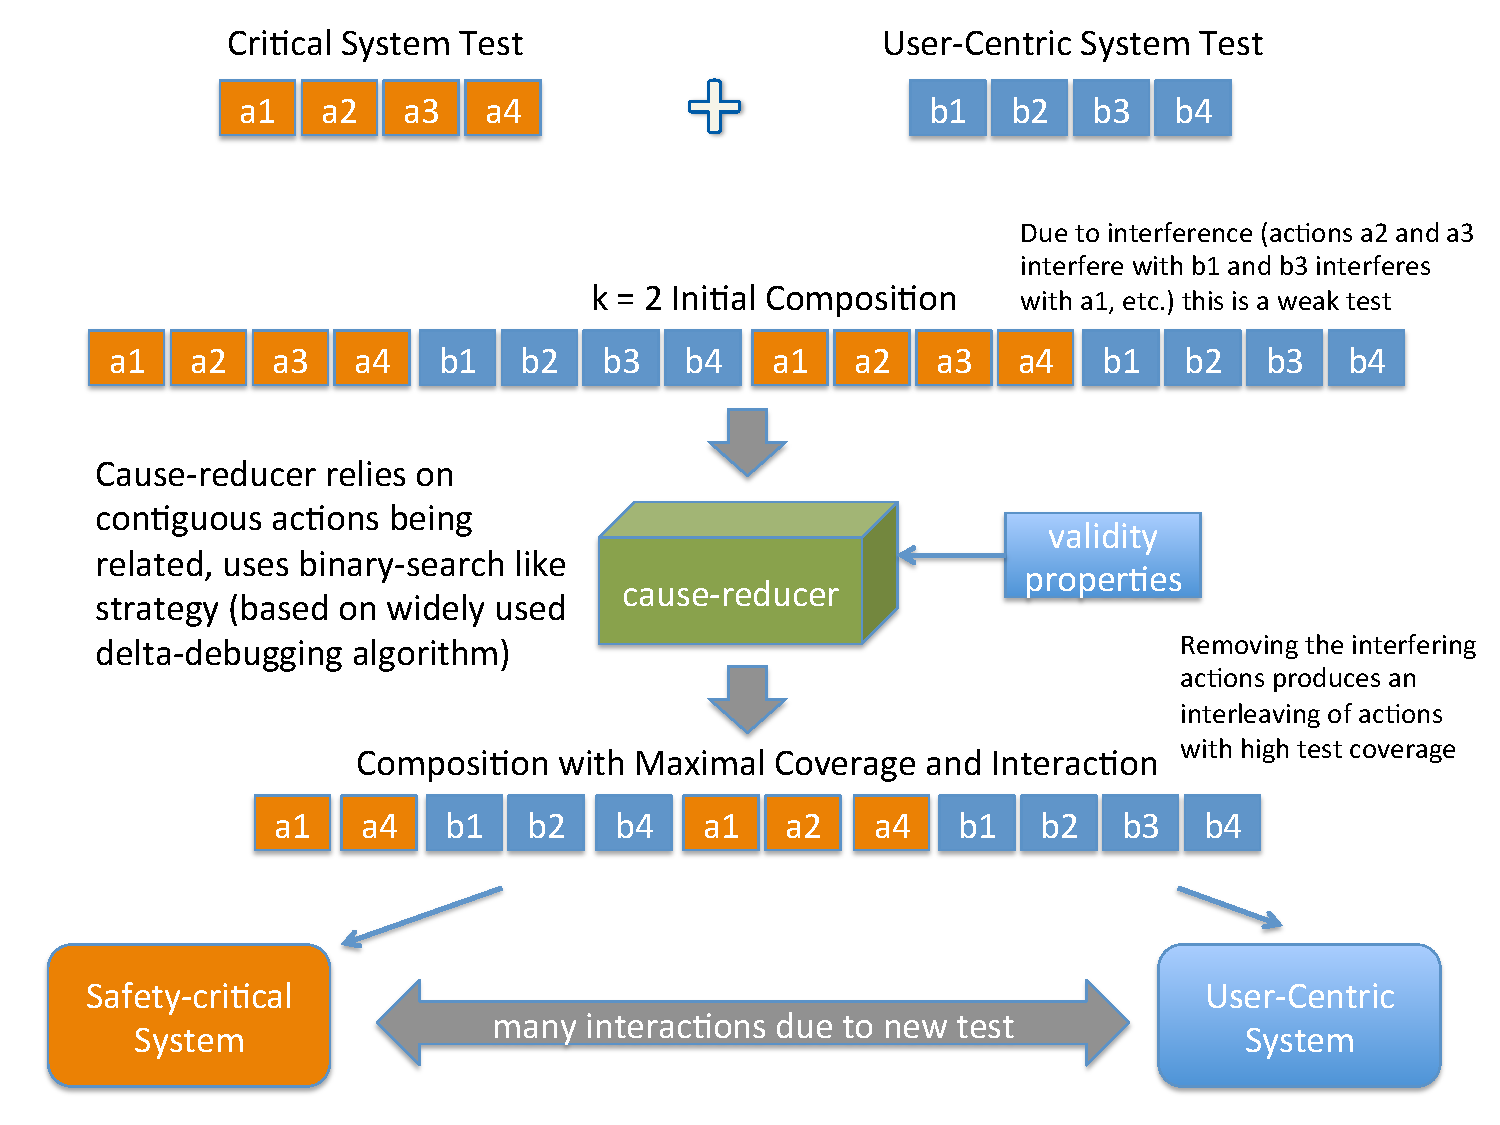
\includegraphics[width=0.6\columnwidth]{testcomp}
\caption{Composition of heterogeneous system test cases.}
\label{fig:compose}
\end{figure}


\mycomment{
To understand the concept, consider the simple case where {\tt A =
  a1.a2.a3.a4 and B = b1.b2.b3.b4}, with $k = 3$.  If {\tt a1}
interferes with {\tt B}, causing the catalog to fail with an invariant
violated at action {\tt b3}, then our approach can produce a test such
as: {\tt a2.a3.a4.b1.b2.b3.a1.}{\tt a2.a3.a4.b1.b2.b3.b4.a1.a2.a3. a4}. Here,
{\tt a1} is removed from the copy of {\tt A} before any {\tt b3}, but
remains in the final version, from which all {\tt B} actions are
removed, because it adds new code coverage of the low-level file
system.  One {\tt b4} instance is removed, because it causes the
low-level file system code to be in a state such that the second copy
of {\tt B} exercises less code (it forces an early garbage collection
of flash blocks).  Using gains in coverage to change the base test (a
variation of cause reduction we refer to as ``amplification''), we can direct
the reduction toward this high-coverage, valid, composed test without
human intervention.  }

\subsection{Initial Results and Research Problems}

We implemented a simple version of our approach in the TSTL tool for
Python testing \cite{NFM15}, and applied
it to compose tests for the widely used {\tt pyfakefs} file system.  We generated a
large set of tests containing only file operations and a large set of
tests containing only directory operations, and then applied both a
n\"aive composition approach and a simple version of our approach
(without amplification), with increasing $k$.  Directory-only tests
had a mean branch coverage of 343.3 branches, and file-only tests had
a mean branch coverage of 612.03 branches.  N\"aive composition
improved this to 651.87 mean branches, but $k=2, 3, 4$ composition improved
the means to 693.23, 698.3 and 714.37 mean branches, respectively.
All results were statistically significant, and at $k=4$, produced
tests were highly complex and using chunks of original tests as
``components'' of complex file system operations not present in either
set of simpler tests.

\mycomment{
Because this approach suggests that test composition is essentially a
search problem, an obvious question is why we use cause
reduction/delta-debugging rather than a more traditional search-based
evolutionary or genetic algorithm approach \cite{searchtest,McMinn04search-basedsoftware,FA11}.  First, we believe that
removal of operations is the only mutation of interest in this
context: crossover or random change in test actions is likely to
introduce invalid test behavior.  Our assumption is that tests to be
composed are valid in isolation, and only nearby behaviors are of
interest (or likely to maintain single-component validity).  Second,
many search-based techniques expect access to branch distances and
other intrusive instrumentation.  This may not be feasible for
embedded systems; we can use cause reduction with instrumentation only
for user-centric code or, in the worst case, for neither system.  This
necessitates guidance by other means.}

The sketch of a composition approach here is, of course, highly
incomplete. We must determine, for example, how best to choose initial
values for $k$, how to identify and make modifications to
delta-debugging that speed termination of the search or allow for
better parallelization, and how to devise heuristics for abandoning a
failing search and using a larger $k$.  Other basic research questions
are numerous: e.g., is it best to first amplify for coverage, then
search for faults, or is this inefficient? For some systems composition
of more than two tests may be essential to exploring interactions.
However, composing more than 4-5 tests may make cause reduction
prohibitively expensive.  Does composition compose?  That is, for
truly first-class tests we would expect that {\tt (A+B) + (C+D) =
  A+B+C+D} but this is far from clear in the context of test
composition, where {\tt C} and {\tt B} may have unavoidable
interference.  Another key research issue is how to extend the number
of cases where composition can succeed.  In some cases, composition of
two tests cannot proceed without ``bridging'' actions contained in
neither test.  Some bridging actions may be possible to generate
automatically, through static analysis of tests (variable renamings,
object creation and deletion, etc.), or via the same term rewriting
approach taken in normalization.  Others may require generating
random actions that cause reduction can discard if they are not needed
or are interfering.  We expect that other complexities will arise
during experimentation.

{\bf Deliverables:}  We will develop fully documented tools to support automated
composition of tests for components of CPS.  These tools will include
both TSTL-based pushbutton tools for Python based automated
testing and frameworks for application to general, custom CPS, allowing
engineers to define test decomposition and validity properties.

\bibliographystyle{abbrv}
\bibliography{bibliography}

\end{document}
